\documentclass{article}
\usepackage[utf8]{inputenc}
\usepackage{amsmath}
\usepackage{xcolor}
\usepackage[top=2cm, bottom=2cm, left=2cm, right=2cm]{geometry}
\setlength\parindent{0pt}

\usepackage{listings}
%\usepackage{color}
\usepackage{graphicx}
\usepackage{float}
\usepackage{caption}

\usepackage{verbatim}
\let\oldv\verbatim
\let\oldendv\endverbatim

%\userpackage{minted}

\definecolor{dkgreen}{rgb}{0,0.6,0}
\definecolor{gray}{rgb}{0.5,0.5,0.5}
\definecolor{mauve}{rgb}{0.58,0,0.82}
\definecolor{light-gray}{gray}{0.95}


\lstset{frame=tb,
  language=Java,
  aboveskip=6mm,
  belowskip=6mm,
  showstringspaces=false,
  columns=flexible,
  basicstyle={\small\ttfamily},
  numbers=none,
  numberstyle=\tiny\color{gray},
  keywordstyle=\color{blue},
  commentstyle=\color{dkgreen},
  stringstyle=\color{mauve},
  breaklines=true,
  breakatwhitespace=true,
  tabsize=3,
  backgroundcolor=\color{light-gray},
  language=Matlab
}

%\usepackage{natbib} replaced by line below to make refernces work
\usepackage[square,sort,comma,numbers]{natbib}
\usepackage[nottoc,numbib]{tocbibind} %to get references in table of contants
\usepackage{graphicx}

\usepackage{bm}

\usepackage{hyperref}
\hypersetup{
	colorlinks,
	citecolor=black,
	filecolor=black,
	linkcolor=black,
	urlcolor=black
}

\usepackage{mdframed}
\usepackage{lipsum} % for creating dummy text
\mdfdefinestyle{MyFrame}{%
	linecolor=black,	
	backgroundcolor=gray!20!white,
	skipbelow = 8mm,
	skipabove = 8mm}

\usepackage{scrextend}

\usepackage{multimedia}
\usepackage{media9}

\title{Fys4150\\Project 3\\ }
\author{Peter Killingstad and Karl Jacobsen\\
\\
\url{https://github.com/kaaja/fys4150}}
\begin{document}
	
\maketitle



\section*{Note to instructurs reagarding Github repository}
If the above Github-link does not work, it is eighter because you have not yet accepted our invite to the repository, or you have not yet provided us with an e-mail addres available at Github so that we can invite you. The Github user you will be invited from is "kaaja". If the latter applies to you, please send us an e-mail with an e-mailadress available in Github or your Github username so that we can send you an invite. Our e-mailadresses: peter.killingstad@hotmail.com, karljaco@gmail.com.



\section*{Abstract}
Systems of 2nd order ordinary differential equations (ODEs), describing planetary motion, are scaled and reduced to 1st order ODEs. The equations are discretized using forward Euler's method and the Velocity Verlet method, and implemented in C++ by use of classes and class inheritance. The methods are shown to involve approximately the same number of FLOPS. Velocity Verlet is shown to be the only method the preserves energy and angular momentum well, and is also higher in convergence rate order compared to forward Euler. Both methods produces reasonable planetary orbits in a two body system consisting of the sun and the earth. The velocity Verlet method reproduces exact terminal velocities for the earth, under different assumptions on the gravity force, and also gives reasonable results in a three body system both with a stationary and non-stationary sun is modelled. The full solar system is well approximated with Velocity Verlet. The observed perihelion precession of Mercury around the sun is well reproduced by adding a relativistic correction in the gravitational force.


\section{Introduction}
Multibody systems governed by coupled 2nd order ordinary differential equations (ODEs) appear several places in physics, among other places in mechanics and astrophysics. Systems like these can be simplified by variable subsitution, leading to a larger system of only 1st order ODEs. This technique is demonstrated and applied here.\\

Often the more general a method is, the more useful it is. In this project, which deals with planetary orbits, the equations are scaled to astronomical units. In addition to making the equations easier to work with, the scaling also makes the equations and their solutions more general and potentially applicable to other physical problems without the need to do large changes to the computer programs. In addition scaling was necessary in this case, since use of SI units probably would lead to numerical problems with overflow.\\

Solving large systems like these cannot be done analytically, and must be done numerically. Several methods are available for calculating derivatives that appears in the equation system. Knowledge about the properties of the different methods is crucial for getting quality solutions. There are several examples where lack of knowledge about numerical methods has led to dissasters in the real world. In this project we use the forward Euler method and Velocity Verlet method, and it is shown that the Forward Euler method do not obey basic physical properties such as energy and angular momentum preservation. Also it is shown that the speed of convergence of the Velocity Verlet method is twice that of Forward Euler.\\

Working with many equations on the computer, can increase the probability of errors lik e.g. typing errors dramatically. Methods that reduces the probability of such errors are essential for efficient and correct solutions. In physical systems like we are dealing with here, coupled 1st order ODE systems, most of the equations are almost identical. A perfect programming method for dealing with such cases are classes. With classes, one typically writes many equations that is almost identical only once. This reduces the probability of typing errors considerably! Classes is used extensively in this project.\\

In this project we will deal with some special situations, like introduction of a relativistic correctional term to the gravitational force on Mercury (for calculation of the periihelion precession) and other alternative gravitational forces. Introduction of such modifications can be dealt with more smoothly, compared to adding lots of if-tests inside the classes, by utlizing class inheritance. With class ineritance, one simply construct new classes that inherits all the property of the old classes and then make simple changes to new class. This method potentially increases the readability and generality of the code, the last part implying that it can be used easier with other problems.\\

It is easy to lose control of where problems occours and how the different parts of the program works when solving large systems. Solving the full problem directly one quickly ends up with problems localizing errors, since it is hard to find errors in large systems. A step-wise implementation, incorporating only parts of the system at a time and checking different aspects at the different steps, increases the model users knowledge about the full program and system. This step wise approach is implemented in this project. Several tests from the step wise implementation is reported.\\

First a two-body system with only the sun and the earth, where the sun is stationary, is solved. On this system several things are tested: The performance of the solvers and the escape velocity for different gravitational forces. Then a three-body system is introduced, where checking for the effects of the mass of the third planet on the orbits. Finally a real center of mass system with a moving sun is introduced in the three body system, before the full solar system is simulated. The perihelion precession of Mercury around Sun is simulated as an end test of the precission of the program.\\

The next sections of the report describes the data, the equations and shows the scaling of these, in addition to describing the main idea of our class setup. The results section includes all results, while the final section deals with conlcusions and discussion of limitations.


\section{Data}

\subsection{Data sources}
All data are taken from the NASA's page \href{{http://ssd.jpl.nasa.gov/horizons.cgi#top}}{\nolinkurl{http://ssd.jpl.nasa.gov/horizons.cgi\#top}}.\\

From the above page we manually extract initial positions and velcocities from all planets and the sun. These data are pasted into the file "dataProject3", which can be found in the Github-repository.\\

When using the mentioned webpage from NASA, we change from \textbf{OBSERVER} to \textbf{VECTOR}. We extract velocities in units of AU per day, and then manually transform this into AU per year. All manipulations done with the initial data leading to the final datafile "dataProject3" that is used, can be found in the file "dataFileProj3calculations.ods" in the repository.

\subsection{Replication information}
Replicability is very important in science. Without this, it is hard to judge the quality of the results. Also, with a high level of replicability, it is very easy for other people to build on the work direclty. In this project, we have made a python file which can be used to reproducde every figure and result in this report. Below follows the details on how to reproduce the different figures.\\

When the repository is pulled, the following commands from the terminal can be used.

\begin{itemize}
	\item  \colorbox{gray!30}{python runProject3.py --twoBodyFEuler} Figures 3, 5, 7, 9, 11, 13, 17\\
	
	\item  \colorbox{gray!30}{python runProject3.py --twoBodyVelocityVerlet} Figures 4, 6, 8, 10, 12, 14, 16, 18\\
	
	\item  \colorbox{gray!30}{python runProject3.py 	--terminalVelocity} Figure 19\\
	
	\item  \colorbox{gray!30}{python runProject3.py --terminalVelocityAlternativeForce} Figures 20, 21, 22\\
	
	\item  \colorbox{gray!30}{python runProject3.py --threeBodyFixedSun} Figure 23\\
	
	\item  \colorbox{gray!30}{python runProject3.py --threeBodyFixedSunJupiter10} Figure 24\\
	
	\item  \colorbox{gray!30}{python runProject3.py --threeBodyFixedSunJupiter1000} Figures 25\\
	
	\item  \colorbox{gray!30}{python runProject3.py --threeBodyMovingSun} Figure 26\\
	
	\item  \colorbox{gray!30}{python runProject3.py --threeBodyMovingSunJupiter10} Figure 27\\
	
	\item  \colorbox{gray!30}{python runProject3.py --threeBodyMovingSunJupiter1000} Figure 28\\
	
	\item  \colorbox{gray!30}{python runProject3.py --solarSystemMovingSun} Figure 29\\
	
	\item  \colorbox{gray!30}{python runProject3.py --solarSystemMovingSunInnerPlanets} Figure 30\\
	
	\item  \colorbox{gray!30}{python runProject3.py --perihelion} Figure 31
\end{itemize}


\section{Theory}

\subsection{Order reduction}
Lets describe the general procedure for reducing a 2nd order ODE to a 1st order system of ODEs. Say we have an equation describing Newton's 2nd law:

\begin{equation}
F/m = a = \frac{d^2}{dx^2} = -kx
\end{equation}

Now make the "substitutions" $\frac{d^2x}{dt^2} = v$ and $v = \frac{dx}{dt}$ to get the system

\begin{subequations}
	\begin{align}\label{eq:dxdt}
	\frac{dx}{dt} &= v
	\end{align}
	
	\begin{align}
	\frac{dv}{dt} &= \frac{d^2x}{dt^2}\\
	 &= \frac{F}{m}\label{eq:dvdt}
	\end{align}
\end{subequations}

In the above the 2nd order ODE is reduced to the system (\ref{eq:dxdt}) and (\ref{eq:dvdt}). Actually, this method can be used to reduce any higher order equation to a system of 1st order ODEs! The solar system is described with Newton's 2nd law, so the reduction of order for the ODEs for the solar system follows the same recepie as listed above.\\

\subsection{Numerical schemes}
Now for the numerical scehmes, forward Euler and Velocity Verlet. Both these methods are derived from Taylor polynomials. The strength of these polynomials is that one has control over the order of the truncation error, the error one gets by truncating the Taylor series to get the wanted approximation. \\

For the forward Euler method, a Taylor expansion around the point $x + h$ is done for $x$ and $v$, and one obtain the discretized system

\begin{subequations}
	\begin{align}
		x_{i+1} = x_i + hv_i + \mathcal{O}(h^2)\label{eq:fev}
	\end{align}
	
	\begin{align}
		v_{i+1} = v_i + ha_i + \mathcal{O}(h^2)\label{eq:fea}
	\end{align}
\end{subequations}

We see from (\ref{eq:fev}) and (\ref{eq:fev}) that the truncation error is of order $h^2$. However, the above is repeated $N$ times, there are $N$ time steps, to get the full solution. Since $h$ is proprtional to $N^{-1}$ ($h = T/N$), the global error goes like $\mathcal{O}(h)$. The forward Euler method is conditionally stable, meaning that is stable only for certain $\Delta t$.\\

The velocity Verlet method is constructed in the same way as the forward Euler method, applying Taylor polynomials. However, a more clever manipulation of the Taylor polynomials is applied, and one ends with

\begin{subequations}
	\begin{align}
	v_{i+1} = v_i + h/2(a_{i+1} + a_i + \mathcal{O}(h^3)\label{eq:vvv}
	\end{align}
	
	\begin{align}
	x_{i+1} = x_i + hv_i + \frac{h^2}{2} a_i + \mathcal{O}(h^3)\label{eq:vvx}
	\end{align}
	
	\begin{align}
	a_i = F_i/m\label{eq:vva}
	\end{align}
\end{subequations}

In the above one must update position before velocity, since we need the acceleration on the current and next step to get the velocity. Calcuating x first, we can insert this into the equation for a, and then we calculate v. We observe that the truncation error, and hence the also the global error, is one order higher compared to forward Euler. This method is unconditionally stable, meaning it is stable for all $\Delta t$. In addition, this method conserves energy better then Forward Euler.

\subsubsection{Algorithm Velocity Verlet and FLOP count}

The velocity Verlet method is implemented with the following algorithm

\begin{lstlisting}
for time in [0,...,T]:
	1) Make acceleration vector
	for planet in planets: 
		accVec[planet] = F[planet]/mass[planet]
					
	2) Calculate position
	for planet in planets: 
		x += hv + h^2/2 accVec[planet]
		
	3) Update vector with old accelerations
	accVecOld = accVec
	
	4) Calculate new acceleration
	for planet in planets: 
		accVec[planet] = F[planet]/mass[planet]
		
	5) Calculate velocity
	for planet in planets:
		v += v + h/2(accVecOld[planet] + accVec[planet]])			
\end{lstlisting}

Now we will count the FLOPS of the above algorithm. For reference, accelerations are calculated with the following formulae

\begin{lstlisting}
rPlanetDistance = getRadialDistance(*planets_[planetNumber]); 

accelerationX_ += -FourPi2*planets_[planetNumber]->getMass()/planets_[0]->getMass()*(xPosition - planets_[planetNumber]->getXPosition())/pow(rPlanetDistance,3);
\end{lstlisting}

From the above listing, we get that each acceleration calculation involves $1(+=) + 1(fourPi2+planets_) + 1(fourPi2+planets_/planets_[0]->getMass) + 1(fourPi2+planets_/planets_[0]->getMass*(xPosition - planets_)) + 1(xPosition - planets_)+ 3(.../r^3) = 8\; FLOPS$.\\

With P denoting the number of planets, N denoting the number of time steps, and the use of the result above for FLOPS per acceleration calculation, the above algorithm gives the following FLOP count for the Velocity Verlet algorithm

\begin{itemize}
	\item  1) $P*(F)_{FLOPS} = P*8\; FLOPS$
	
	\item 2) $P*[1(+=) + 1(+hv) + 1(hv) +2(h^2) + 1(h^2/2) + 8 (F)] = 14 P \; FLOPS$
	
	\item 3) 0 FLOPS
	
	\item 4) Same as 1): $8P\; FLOPS$
	
	\item 5) $P[1(+=) + 1(h/2) + 1(accVecOld + accVec) + 1(h/2*(accVecOld + accVec)] = 4P\;FLOPS$
	
	\item SUM 1) - 5) = 34 P FLOPS
	
	\item TOTAL FLOPS = SUM*N = 34 P N FLOPS $\approx \mathcal{O}(N)\;FLOPS$
\end{itemize}

The above is not fully exact, as how one implements e.g. $4 \pi^2$ into the program affects the FLOP count. However, all necessary terms of the implemented algorithm should be included for the above count to give a correct order, which is $\mathcal{O}(N)\;FLOPS$. Also, in the program x and y are separated, so we get twice as many FLOPS as calculated above. Once again, this does not effect the order properties of the FLOPS, which will be analyzed.\\

We will not do an explicit FLOP count for Forward Euler, which is easier to count for. However, the method for counting FLOPS for Forward Euler is the same as the one applied above. From the lectures, we know that also forward Euler is $\mathcal{O}(N)$ when it comes to FLOPS, with only a few FLOPS less than Velocity Verlet.



\subsection{The solar system equations}
We describe the solar system by Newton's 2nd law assuming circular orbits when scaling and Newton's gravitational law, which for two objects are

\begin{equation}
F_G = M_{earth}\frac{v^2}{r}\label{eq:newtonCircle}
\end{equation}

\begin{equation}
F_G = \frac{GM_{sun}G_{earth}}{r^2}\label{eq:newtonGravity}
\end{equation}

Dividing both equations above by $M_{Earth}$ gives

\begin{equation}
a = \frac{v^2}{r}\label{eq:newtonCircle2}
\end{equation}

\begin{equation}
a = \frac{GM_{sun}}{r^2}\label{eq:newtonGravity2}
\end{equation}


To make the equations simpler, and also to avoid overflow issues that potentially would occour if we had used SI units, we now scale the equatons to Astronomical units to get $v = \frac{2\pi r}{T} = \frac{2\pi Au}{Yr}$. Inserting this scaling into the above system gives

\begin{equation}
a = \frac{2^2 \pi^2 Au^2}{Au\;Yr^2}\label{eq:newtonCircle3}
\end{equation}

\begin{equation}
a = \frac{GM_{sun}}{Au^2}\label{eq:newtonGravity3}
\end{equation}

Setting the above two equations equal and solving for $GM_{sun}$ gives

\begin{equation}\label{eq:GMSun}
GM_{Sun} = 4 \pi^2 (Au)^3/Yr^2
\end{equation}

Now we can insert (\ref{eq:GMSun}) into (\ref{eq:newtonGravity2}) to get

\begin{equation}
a = -\frac{4 \pi^2}{r^2}
\end{equation}

For the x-component we get
\begin{subequations}
	\begin{align}\label{eq:ax}
		a_x &= -\frac{4 \pi^2}{r^2} \cos(\theta)\\
		&= -\frac{4 \pi^2}{r^2 r} r\cos(\theta)\\
		&= -\frac{4 \pi^2}{r^3} x
	\end{align}
\end{subequations}

The same type of calculation gives the y-component. \\

The next step is to add a planet to the system. This will add a new force between earth and the new planet, in addition to the force between the sun and the planets. The force between earth and the new planet will be of the exact same kind as the force between earth and sun, given in (\ref{eq:newtonGravity}). The x accleration term (\ref{eq:ax}) for the earth will now be

\begin{equation}\label{eq:3rdPlanet}
a_x = -\frac{4 \pi^2}{r_{earth,sun}^3} (x_{earth}-x_{sun}) - \frac{4 \pi^2 \frac{M_{jupiter}}{M_{sun}}}{r_{earth,jupiter}^3}(x_{earth}-x_{jupiter}),
\end{equation}

where we see that the only difference between the two terms are the mass-factor, which in the earth-sun term is one. Now Jupiter will have the same kind of expression as above, only with Jupiter instead of earth in the subscripts. Note the similarity! Adding more planets happens in exactly the same way, nothing new happens! Also we note that the 2nd term will be equall for Jupiter and Earth, which potentially can be taken advantage of when solving the equaions numerically. 


\section{Results}
Before turning to the simulation results, we give a short overview of our class implementation.

\subsection{Class implementation}
The figures below show our class herarcy and the flow-chart.

\begin{figure}[H]
		\centering
		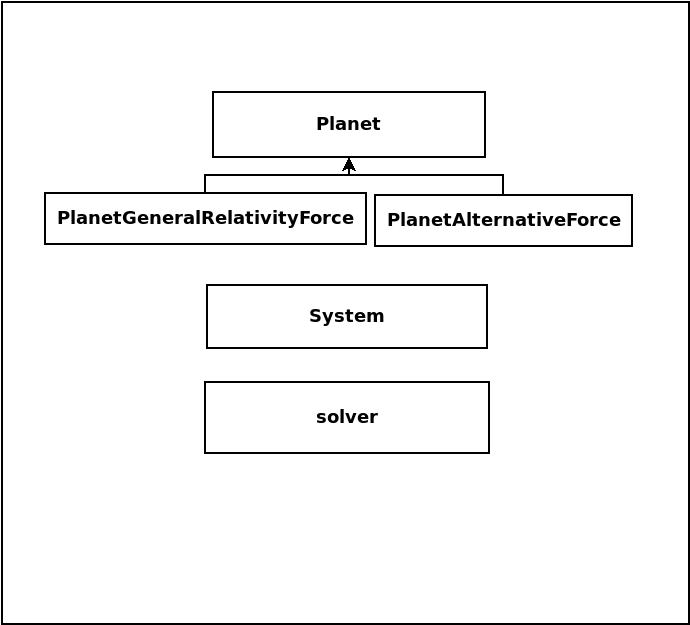
\includegraphics[width=0.6\textwidth]{/home/karl/doc/subj/att/fys4150/project3/resultsKeep/plots/classHiearchy.png}
		\caption{Class hierarcy}
		\label{1}
\end{figure}

\begin{figure}[H]
		\centering
		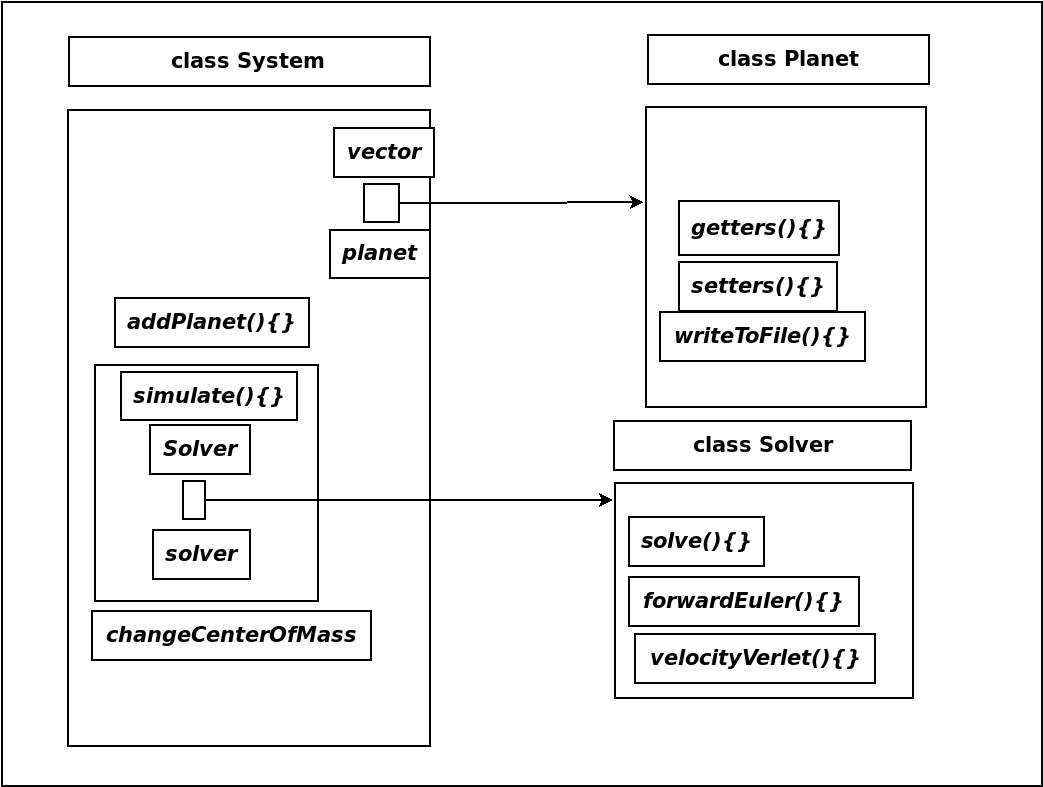
\includegraphics[width=0.6\textwidth]{/home/karl/doc/subj/att/fys4150/project3/resultsKeep/plots/flowChartProject3.png}
		\caption{Flow chart}
		\label{1}
\end{figure}


The class hierarchy figure shows how the program in project3 is divided into different objects. We have a super class "Planet" which defines all properties of a planet. Then we have two subclasses of "Planet" called "planetGeneralRelativity" and "PlanetAlternativeForce".\\ 

The System class contains all planet objects, and the Solver class contains algorithms for solving ODE's. The algorithms in the class are forward Euler and Velocity verlet.\\

The subclasses inherits all the properties of planet, except that their acceleration is changed. For the PlanetGeneralRelativityForce class we have a correction term on the acceleration to get a relativistic gravitational force. In the PlanetAlternativeForce class the acceleration is changed from beeing divided by $r^3$ to $r^{\beta}$, where $\beta \in [2,3]$, to investigate it's impact on the planet system.\\  

In the flow chart figure we can ses the flow of the program. In the class System we have a vector containing objects of the class planets. The planets can be of the type "Planet" or of either one of the subclasses "PlanetGeneralRelativityForce" or "PlanetAlternativeForce".\\ 

Inside the Planet classes we can obtain certain values of the planet by calling on the "get methods". There is also set methods to set velues of the planets. \\

Within the System class we can simulate the planetary system by using the Solver class. Calling the method "simulate" will send all the planet objects to a solver, that solves a system of ODE's for all the planets in the planetary. This is done by either using forward euler method or velocity verlet method, which is specified by the user. 

\subsection{Forward Euler versus Velocity Verlet}

\subsubsection{Positions}
The below figures show the results for the x and y-positions as functions of time, forward Euler to the left and Velocity Verlet to the right. We used the intial position $(x,y) = (1,0)\;Au$ and initial velocity $(v_x, v_y) = (0, 2\pi.)$ for the Earth, with the Sun fixed in the center.


\begin{minipage}{.45\textwidth} 
	\begin{figure}[H]
		\centering
		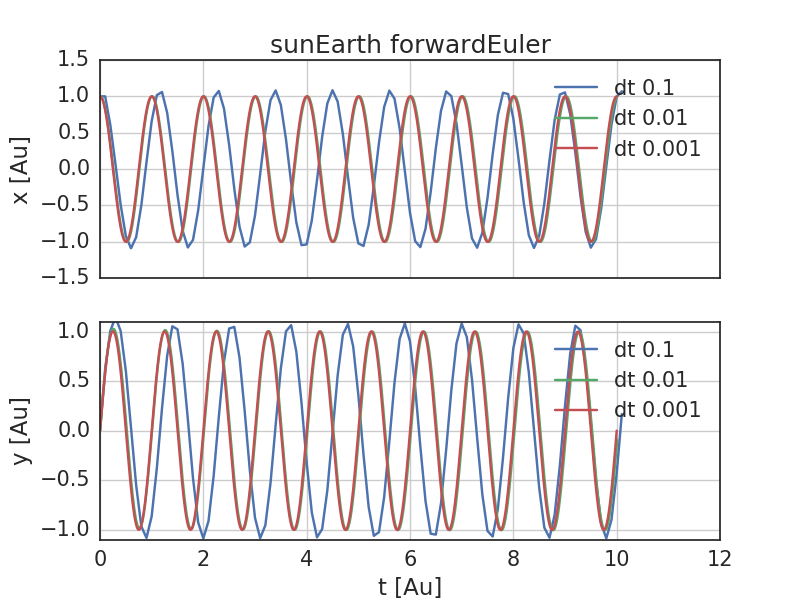
\includegraphics[width=0.99\textwidth]{/home/karl/doc/subj/att/fys4150/project3/resultsKeep/plots/sunEarthTimesForwardEuler.png}
		\caption{Sun-Earth system. Effect of $\Delta t$ over a 10 year period. \\ \textit{The Forward Euler method seems to converge for the two smallest $\Delta t$}}
		\label{1}
	\end{figure}
\end{minipage}\hfill
\begin{minipage}{.45\textwidth} 
	\begin{figure}[H]
		\centering
		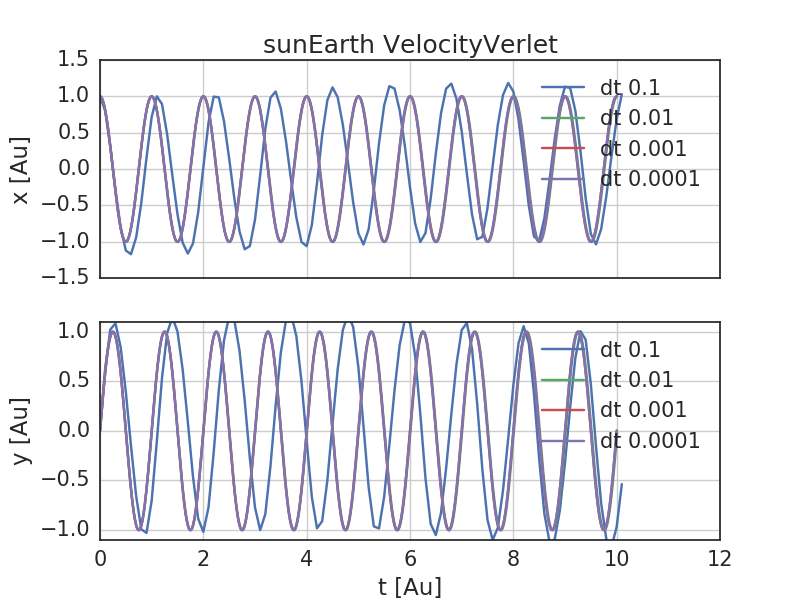
\includegraphics[width=0.99\textwidth]{/home/karl/doc/subj/att/fys4150/project3/resultsKeep/plots/sunEarthTimesVelocityVerlet.png}
		\caption{Sun-Earth system. Effect of $\Delta t$ over a 10 year period. \\ \textit{The Velocity verlet method seems to converge faster than Forward Euler}}
		\label{1}
	\end{figure}
\end{minipage}\hfill
\vspace{2ex}

As can be seen of the figures above, both methods converges when $\Delta t$ is lowered.  Also the Velocity Verlet method seems to converge faster.\\

The next two sets of figures shows the orbits for different $\Delta t$ for the two methods.

\begin{minipage}{.45\textwidth} 
	\begin{figure}[H]
		\centering
		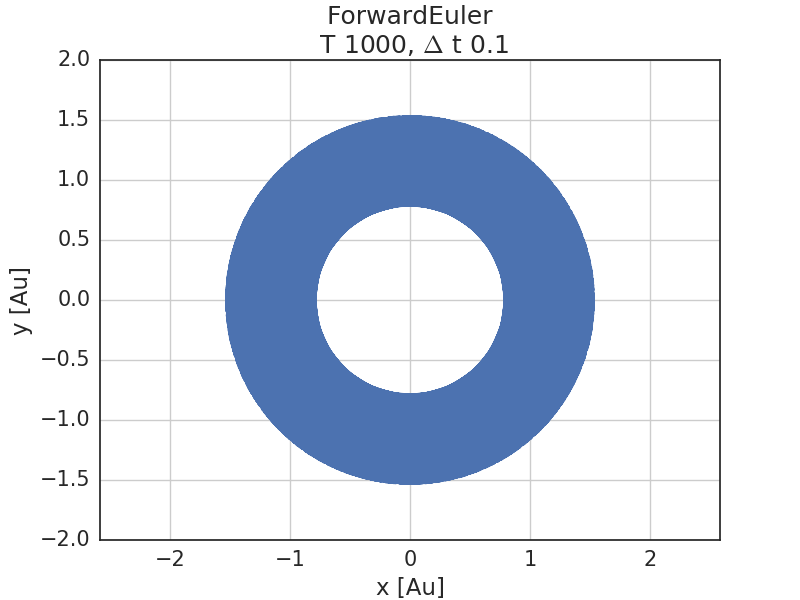
\includegraphics[width=0.99\textwidth]{/home/karl/doc/subj/att/fys4150/project3/resultsKeep/plots/sunEarthfinalTime1000N10000ForwardEuler.png}
		\caption{Sun-Earth system. Forward Euler. 1 000 years \\ \textit{Non-circular orbits when time step is large.}}
		\label{1}
	\end{figure}
\end{minipage}\hfill
\begin{minipage}{.45\textwidth} 
	\begin{figure}[H]
		\centering
		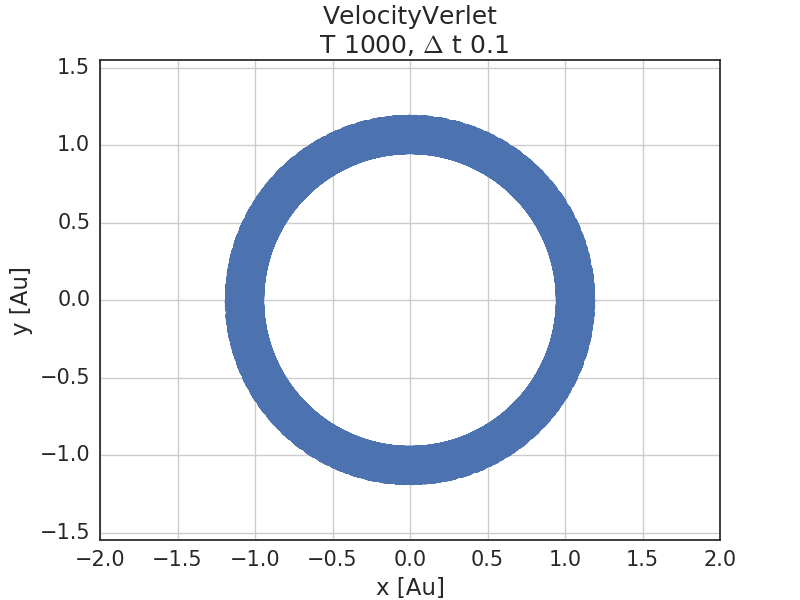
\includegraphics[width=0.99\textwidth]{/home/karl/doc/subj/att/fys4150/project3/resultsKeep/plots/sunEarthfinalTime1000N10000VelocityVerlet.png}
		\caption{Sun-Earth system. Velocity Verlet. 1 000 years. \\ \textit{Large time step gives bad solutions also for Velocity Verlet.}}
		\label{1}
	\end{figure}
\end{minipage}\hfill
\vspace{2ex}

\begin{minipage}{.45\textwidth} 
	\begin{figure}[H]
		\centering
		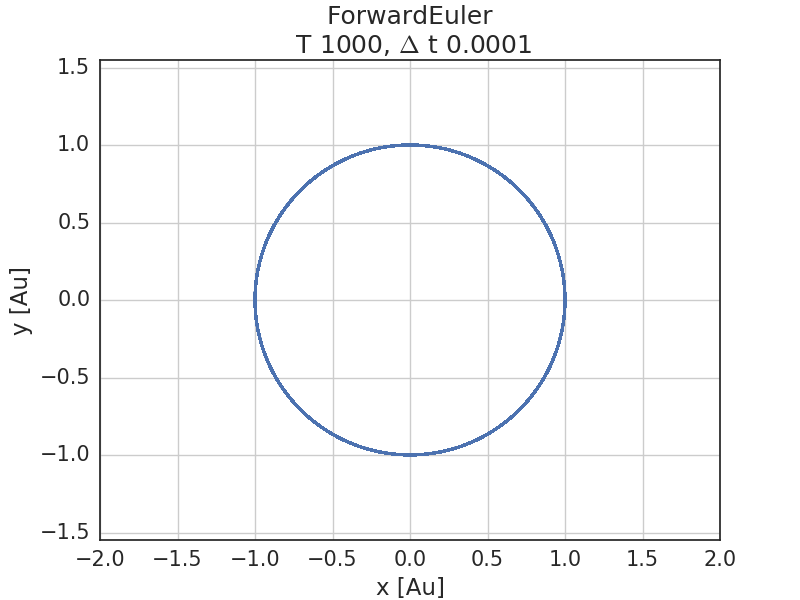
\includegraphics[width=0.99\textwidth]{/home/karl/doc/subj/att/fys4150/project3/resultsKeep/plots/sunEarthfinalTime1000N10000000ForwardEuler.png}
		\caption{Sun-Earth system. Forward Euler. 1 000 years. \\ \textit{For $\Delta t = 0.0001$, the forward Euler seems to give circular orbits.}}
		\label{1}
	\end{figure}
\end{minipage}\hfill
\begin{minipage}{.45\textwidth} 
	\begin{figure}[H]
		\centering
		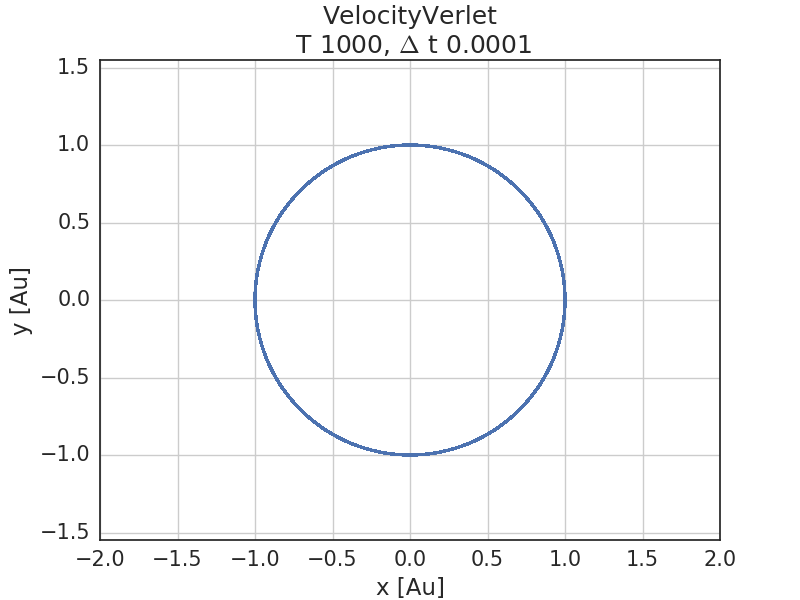
\includegraphics[width=0.99\textwidth]{/home/karl/doc/subj/att/fys4150/project3/resultsKeep/plots/sunEarthfinalTime1000N10000000VelocityVerlet.png}
		\caption{Sun-Earth system. Velocity Verlet. 1 000 years. \\ \textit{The solution looks similar to Forward Euler.}}
		\label{1}
	\end{figure}
\end{minipage}\hfill
\vspace{2ex}

The 2 sets of figures above confirms what we found in the figures with x and y-position agains time: The precision is bettered when $\Delta t$ is lowered. 

\subsubsection{Energy and angular momentum}
Next we analyze the evolution of energy in the numerical solutions. Since all forces in our systems are conservative, meaning that the work done by the forces is path independent, total mecahnical energy, the sum of kinetic and potential energy, should be preserved. Consearvation of energy is a crucial physical principle which we want to maintain in our numerical solutions. The below figures show the difference in total energy compared to the initial total energy, forward Euler to the left and Velocity Verlet to the right.


\begin{minipage}{.45\textwidth} 
	\begin{figure}[H]
		\centering
		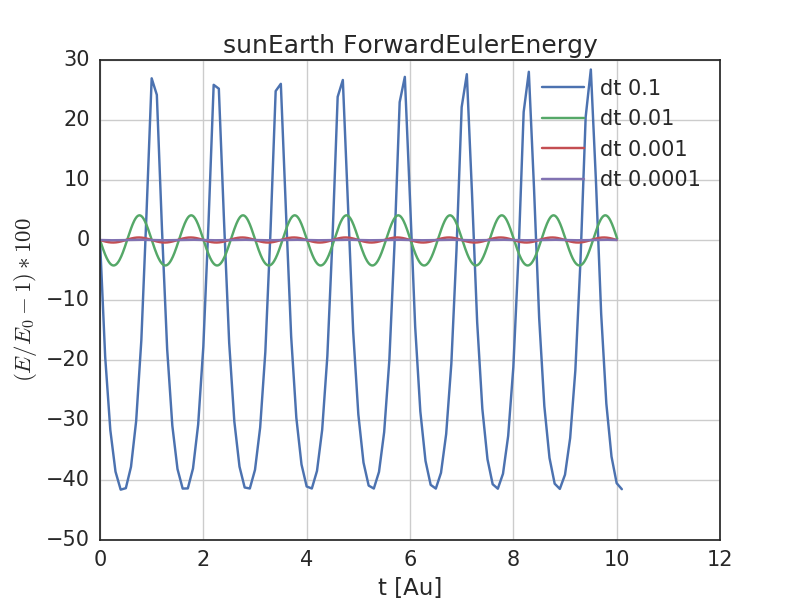
\includegraphics[width=0.99\textwidth]{/home/karl/doc/subj/att/fys4150/project3/resultsKeep/plots/sunEarthEnergyForwardEuler.png}
		\caption{Sun-Earth system. Total Energy change from initial energy, pec centage. Forward Euler. 10 years. \\ \textit{Energy is not preserved with the Forward Euler method}}
		\label{1}
	\end{figure}
\end{minipage}\hfill
\begin{minipage}{.45\textwidth} 
	\begin{figure}[H]
		\centering
		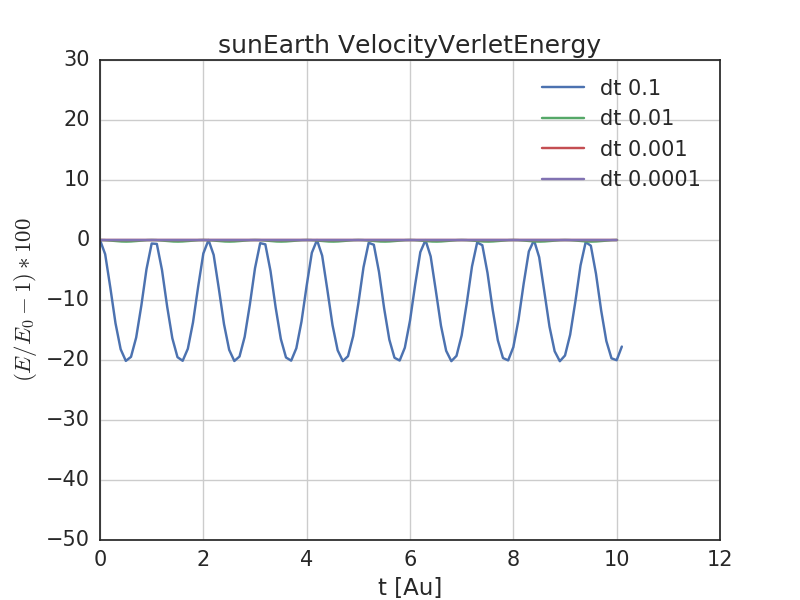
\includegraphics[width=0.99\textwidth]{/home/karl/doc/subj/att/fys4150/project3/resultsKeep/plots/sunEarthEnergyVelocityVerlet.png}
		\caption{Sun-Earth system. Total Energy change from initial energy, pec centage. Velocity Verlet. 10 years. \\ \textit{Energy is preserved better in Velocity Verlet provided fine enough time step. }}
		\label{1}
	\end{figure}
\end{minipage}\hfill
\vspace{2ex}

The two figures above show that for forward Euler, energy can actually increase, even for smaller $\Delta t$. For Velocity Verlet, energy seems to be preserved better compared to Forward Euler. \\

Another important physical property which we want to contain in the numerical simulations, is presevation of angular momentum conservation, $\frac{d \vec{L}}{dt} = \sum_i \vec{r}_i \times \vec{F^{ext}_i} = 0$. There is zero change in angular momentum, since the net external forces are zero. The next figures show the same kind of figures as for energy above, but now for angular momentum. 



\begin{minipage}{.45\textwidth} 
	\begin{figure}[H]
		\centering
		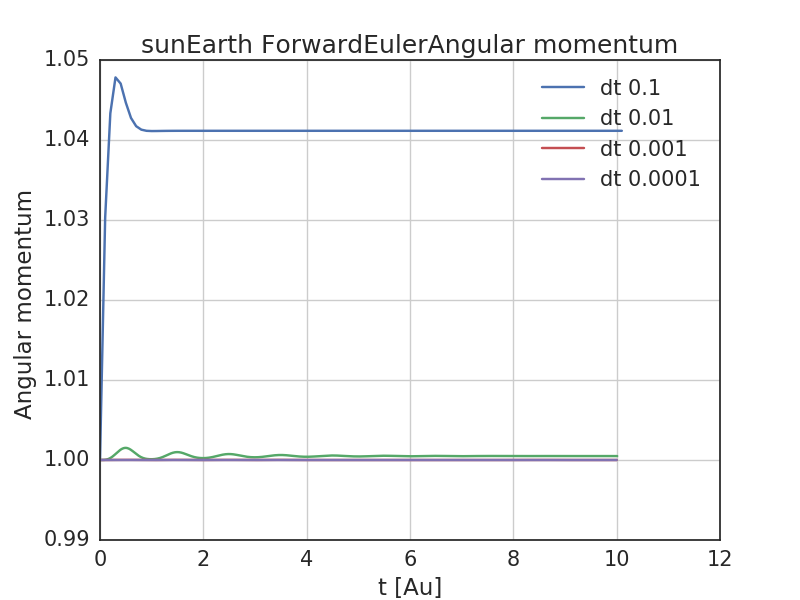
\includegraphics[width=0.99\textwidth]{/home/karl/doc/subj/att/fys4150/project3/resultsKeep/plots/sunEarthAngularMomentumForwardEuler.png}
		\caption{Sun-Earth system. Change angular momentum from initial state, per centage. Forward Euler. 10 years. \\ \textit{Angular momentum seems to be conserverd for the finest time step.}}
		\label{1}
	\end{figure}
\end{minipage}\hfill
\begin{minipage}{.45\textwidth} 
	\begin{figure}[H]
		\centering
		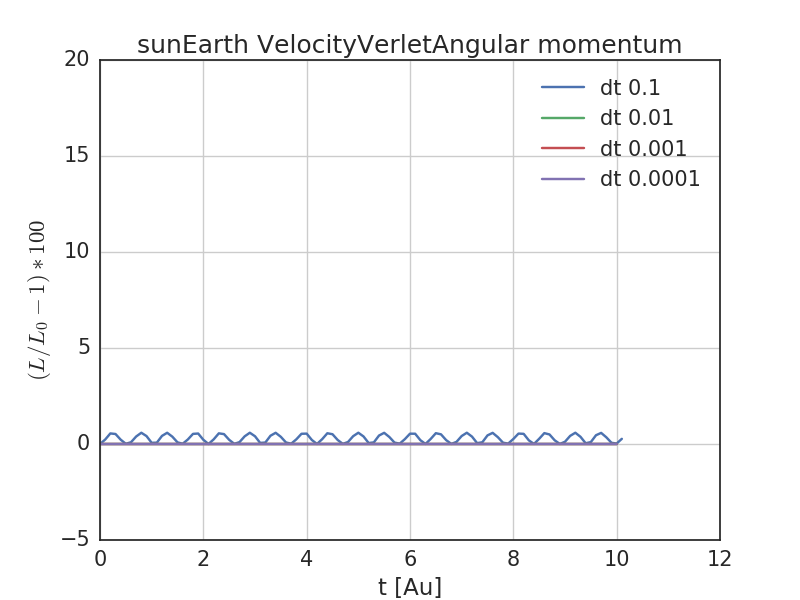
\includegraphics[width=0.99\textwidth]{/home/karl/doc/subj/att/fys4150/project3/resultsKeep/plots/sunEarthAngularMomentumVelocityVerlet.png}
		\caption{Sun-Earth system. Change angular momentum from initial state, per centage. Velocity Verlet. 10 years. \\ \textit{Angular momentum is conserverd given suffiently fine time steps. Conservation achieved faster than with Forward Euler.}}
		\label{1}
	\end{figure}
\end{minipage}\hfill
\vspace{2ex}

The figures above show that as $\Delta t$ gets low, angular momentum is preserved. Also, Velocity Verlet seems to give better angular momentum approximations compared to Forward Euler.\\

Since we know the exact solution for energy and angular momentum, or more precisely, the exact solution for the change, we have constructed a norm measure for computing convergence rates of the schemes. The error-norm is the supremum of the largest difference in energy compared to initial energy. From above we know that the global error's for $x$ and $y$ in Forward Euler should go as respectively $\mathcal{O}(\Delta t)$ and $\mathcal{O}(\Delta t^2)$, so the orders of global errors in position and velocity is always twice as high in the Velocity Verlet method compared to the forward Euler method. \\

Since both energy and angual momentum depend on position and velocity, we expect the convergence rate of norms related to energy and norms related to angular momentum to be twice as high for the Velocity Verlet method compared to the forward Euler method. The figures below show the convergence for the energy norm and the angular momentum norm for Forward Euler and Velocity Verlet.

\begin{minipage}{.45\textwidth} 
	\begin{figure}[H]
		\centering
		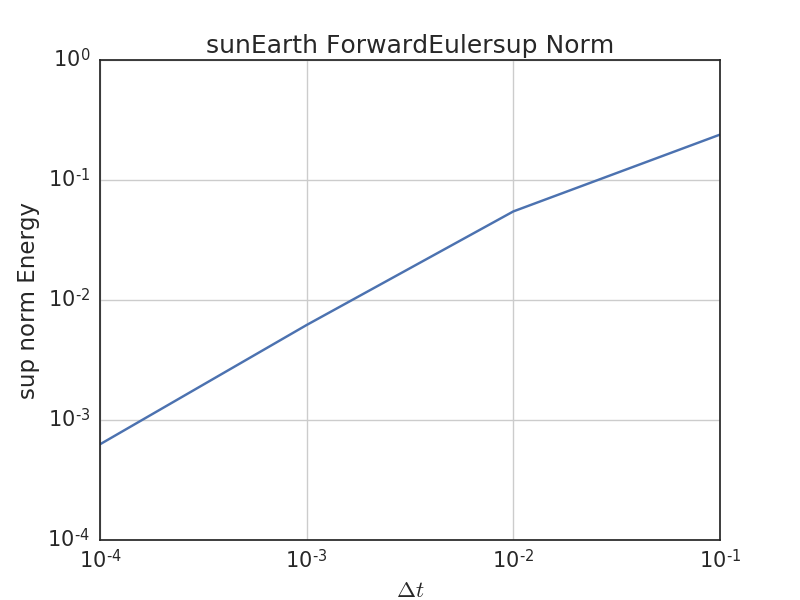
\includegraphics[width=0.99\textwidth]{/home/karl/doc/subj/att/fys4150/project3/resultsKeep/plots/sunEarthsupNormForwardEuler.png}
		\caption{Sun-Earth system. Sup-norm total energy. Forward Euler. \\ \textit{Forward Euler's sup-norm goes like $\mathcal{O}(\Delta t)$}}
		\label{1}
	\end{figure}
\end{minipage}\hfill
\begin{minipage}{.45\textwidth} 
	\begin{figure}[H]
		\centering
		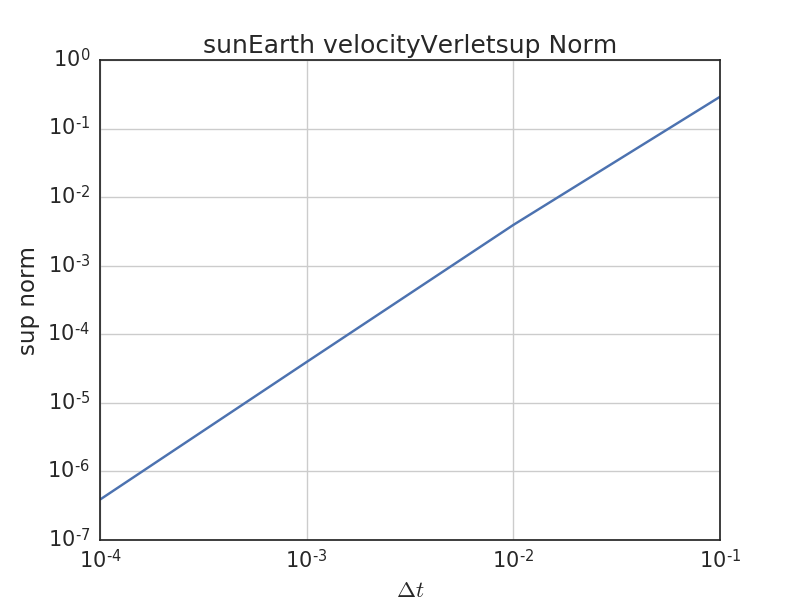
\includegraphics[width=0.99\textwidth]{/home/karl/doc/subj/att/fys4150/project3/resultsKeep/plots/sunEarthsupNormVelocityVerlet.png}
		\caption{Sun-Earth system. Sup-norm total energy. Velocity Verlet \\ \textit{The sup-norm in energy for Velocity Verlet goes one higher order than Forward Euler}}
		\label{1}
	\end{figure}
\end{minipage}\hfill
\vspace{2ex}

\begin{minipage}{.45\textwidth} 
	\begin{figure}[H]
		\centering
		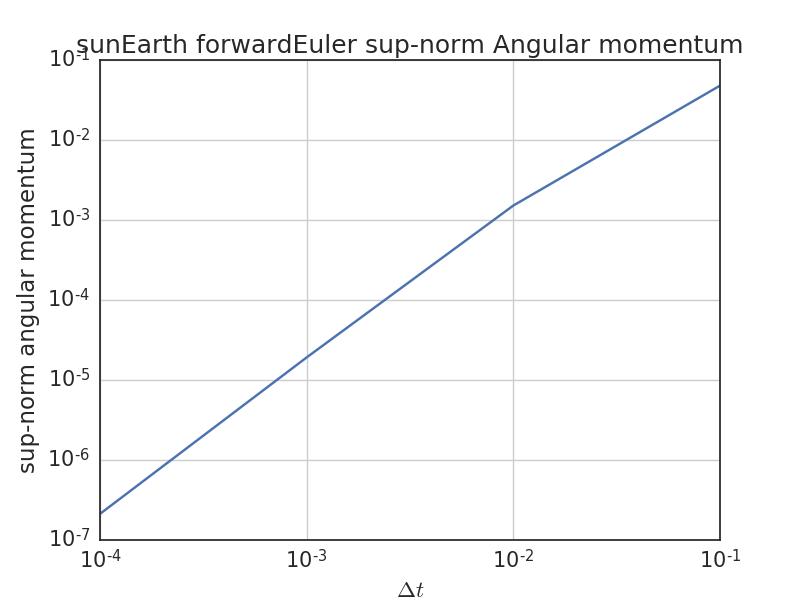
\includegraphics[width=0.99\textwidth]{/home/karl/doc/subj/att/fys4150/project3/resultsKeep/plots/sunEarthsupNormAngularMomentumForwardEuler.png}
		\caption{Sun-Earth system. Sup-norm Angular Momentum. Forward Euler \\ \textit{Forward Euler's sup-norm for angular momentum goes like $\mathcal{O}(\Delta t^2)$}.}
		\label{1}
	\end{figure}
\end{minipage}\hfill
\begin{minipage}{.45\textwidth} 
	\begin{figure}[H]
		\centering
		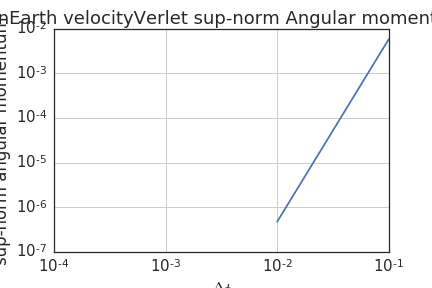
\includegraphics[width=0.99\textwidth]{/home/karl/doc/subj/att/fys4150/project3/resultsKeep/plots/sunEarthsupNormAngularMomentumVelocityVerlet.png}
		\caption{Sun-Earth system. Sup-norm Angular momentum. Velocity Verlet \\ \textit{Velocity Verlet's sup-norm error is $\mathcal{O}(\Delta t^4)$.}}
		\label{1}
	\end{figure}
\end{minipage}\hfill
\vspace{2ex}

The figures on the first row show that the energy norm error goes as 1st order for Forward Euler, while Velocity Verlet goes like 2nd order, so the Velocity Verlet method has twice the convergence rate of forward Euler, as expected.\\

The figures on the 2nd row above show that also for the angular momentum norm, the order for Velocity Verlet is twice that of Forward Euler, as expected.

\subsubsection{Algorithm efficiency}
Knowledge about a methods correctness, discussed above, is crucial, but efficiency is also important. Now we want to see that the efficiency of the algorithms replicate the behaviour we would expect based on the FLOP-count we did in the section "Algorithm Velocity Verlet and FLOP count". In the mentioned section we calculated velocity Verlet to be $\mathcal{O}(N)$ FLOPS. Computational time should be more or less proprtional to FLOPS, so we expect the computational time to be of the same order as the FLOPS. The below figures show the computation time for the methods, forward Euler to the left and Velocity Verlet to the right.

\begin{minipage}{.45\textwidth} 
	\begin{figure}[H]
		\centering
		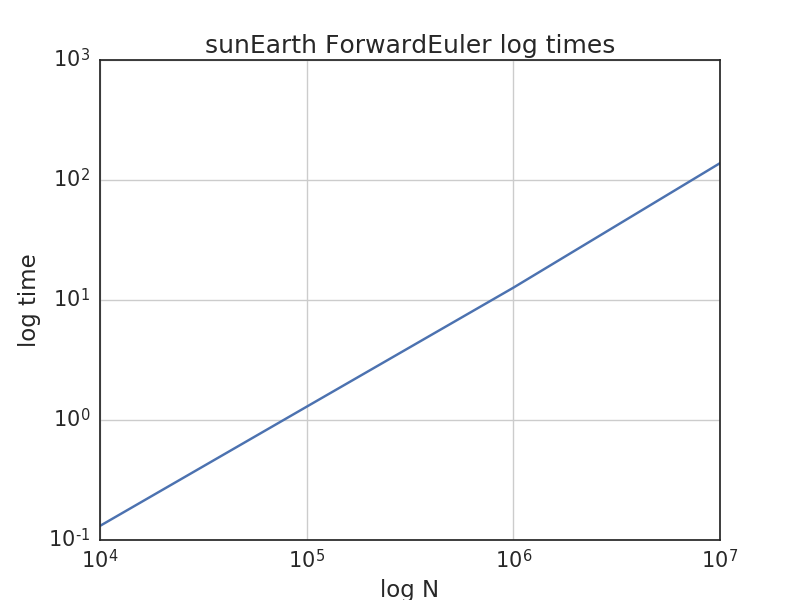
\includegraphics[width=0.99\textwidth]{/home/karl/doc/subj/att/fys4150/project3/resultsKeep/plots/sunEarthlogTimeUsedForwardEuler.png}
		\caption{Sun-Earth system. Log time. Forward Euler \\ \textit{Forward Euler is $\mathcal{O}(N)$}.}
		\label{1}
	\end{figure}
\end{minipage}\hfill
\begin{minipage}{.45\textwidth} 
	\begin{figure}[H]
		\centering
		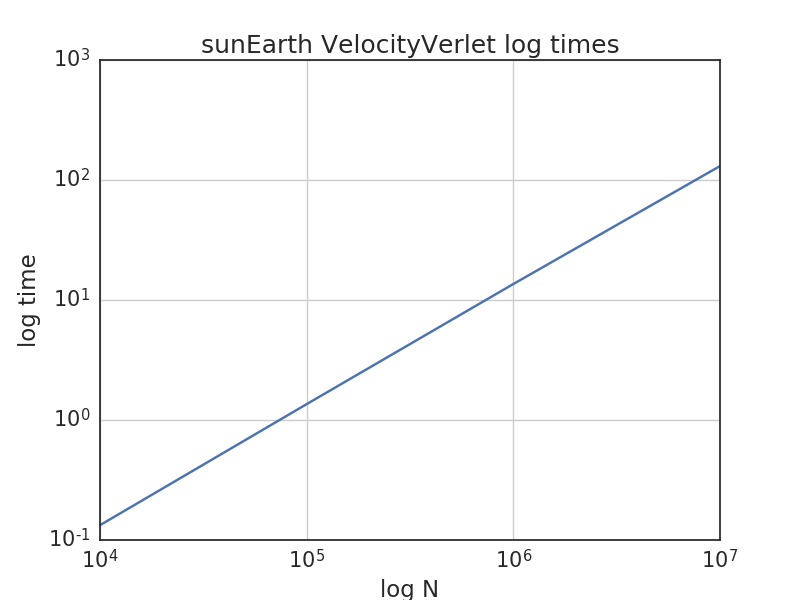
\includegraphics[width=0.99\textwidth]{/home/karl/doc/subj/att/fys4150/project3/resultsKeep/plots/sunEarthlogTimeUsedVelocityVerlet.png}
		\caption{Sun-Earth system. Log time. Velocity Verlet \\ \textit{Velocity Verlet's simulation time is of the same order as Forward Euler.}}
		\label{1}
	\end{figure}
\end{minipage}\hfill
\vspace{2ex}

The two figures above show that the Forward Euler and the Velocity Verlet method both has solution times that is of order 1 in N. This is as expected. 


\subsection{Escape velocity}
Another test to see if the solver obeys the physical laws, is to check if the escape velocity is correct. The escape velcoity equals the velcoity where potential energy equals kinetic energy

\begin{subequations}
	\begin{align}
	E_k  &= E_p \\
	\frac{1}{2} m_E v_{Escape}^2&= \frac{G M_{Sun} M_E}{r_0}\\
	\rightarrow v_E&=\sqrt{\frac{2G M_{Sun} }{r_0}}\\
	&=\sqrt{\frac{2* 4 \pi^2 AU^3 }{AU (Yr)^2}}\\
	&=2 \pi\sqrt{2}\frac{ AU }{(Yr)}
	\end{align}
\end{subequations}

Based on the above equation, we expect the simulations to gove escape when $v > 2\pi \sqrt{2}$. The figures below show the results.

\begin{figure}[H]
	\centering
	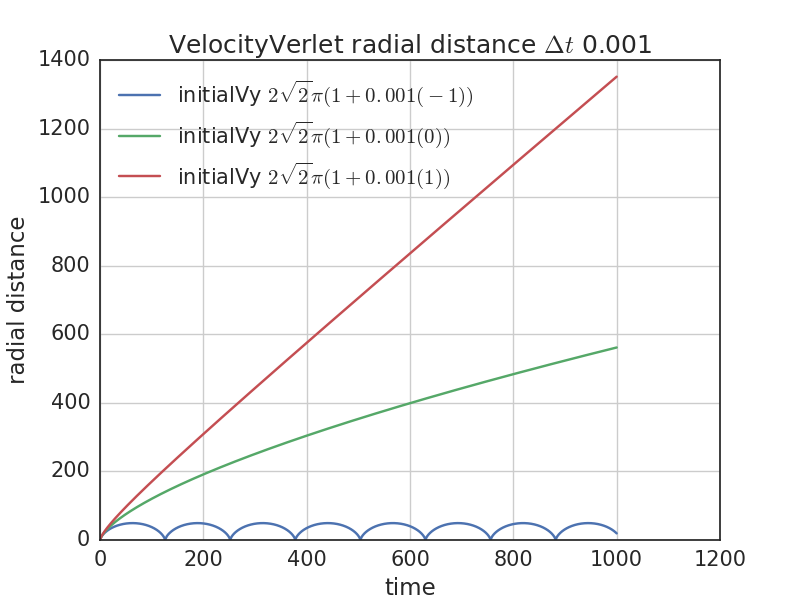
\includegraphics[width=0.6\textwidth]{/home/karl/doc/subj/att/fys4150/project3/resultsKeep/plots/sunEarthTerminalVelocityradialDistanceVelocityVerlet.png}
	\caption{Sun-Earth system. Escape valocity. Radial distance earth sun. \\ \textit{Escape for velocity  $0.1 \%$ higher than $v = 2\sqrt{2}\pi$.}}
	\label{1}
\end{figure}



The figure above show that the simulated escape velocity is very close to the exact terminal velcocity, $2 \pi \sqrt{2}$, supporting the previous results indicating the validity of our solver as a good approximation method.\\

Another test, to see if the numerical solutions corresponds with physics, is to simulate the two planet system with different gravitational forces. We noe assume the gravitational force $F_G = \frac{G M_{Sun} M_{Earth}}{r^\beta}, \beta \in [2,3]$, so that the force is decreased from the original gravitational force when $\beta > 2$. This should give lower escape velocities, since the force is lower. The below figures show escapce velocities for the three different gravitational forces, all forces being lower than the standard force simulated above.


\begin{minipage}{.3\textwidth} 
	\begin{figure}[H]
		\centering
		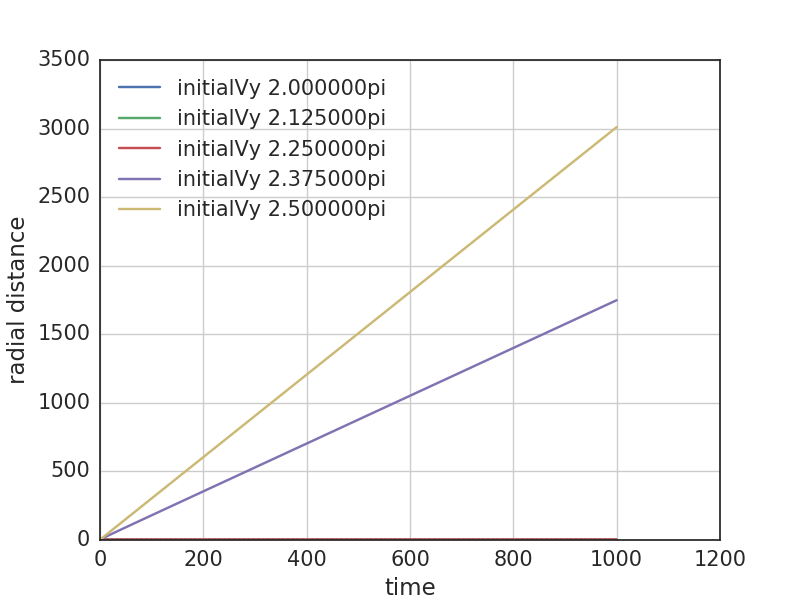
\includegraphics[width=0.99\textwidth]{/home/karl/doc/subj/att/fys4150/project3/resultsKeep/plots/sunEarthradialDistanceVelocityVerletbeta35.png}
		\caption{Sun-Earth system. Alternative force. Escape valocity. $\beta = 2.5$ \\ \textit{Escape velocity is reduced compared to case with normal gravititation.}}
		\label{1}
	\end{figure}
\end{minipage}\hfill
\begin{minipage}{.3\textwidth} 
	\begin{figure}[H]
		\centering
		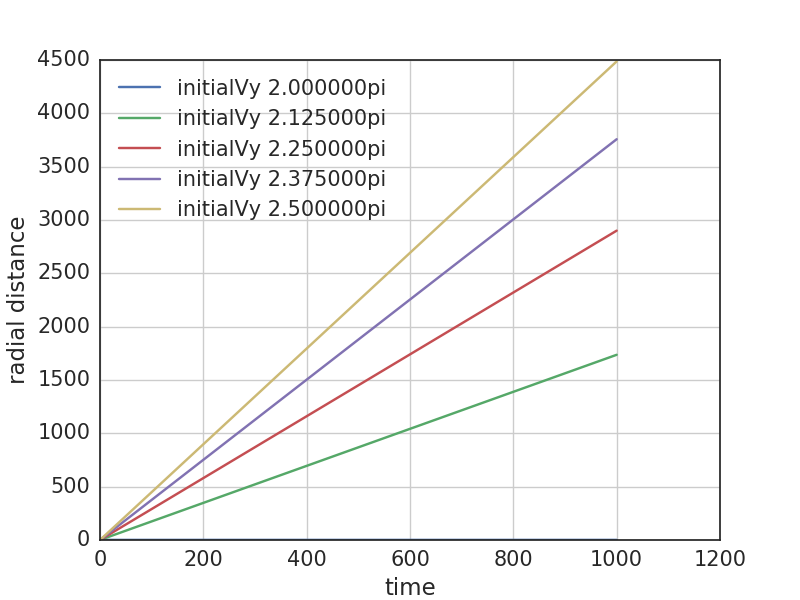
\includegraphics[width=0.99\textwidth]{/home/karl/doc/subj/att/fys4150/project3/resultsKeep/plots/sunEarthradialDistanceVelocityVerletbeta39.png}
		\caption{Sun-Earth system. Alternative force. Escape valocity. $\beta = 2.9$ \\ \textit{The escape velocity is further reduced, and seems to be closer to $2  \pi$}}
		\label{1}
	\end{figure}
\end{minipage}\hfill
\begin{minipage}{.3\textwidth} 
	\begin{figure}[H]
		\centering
		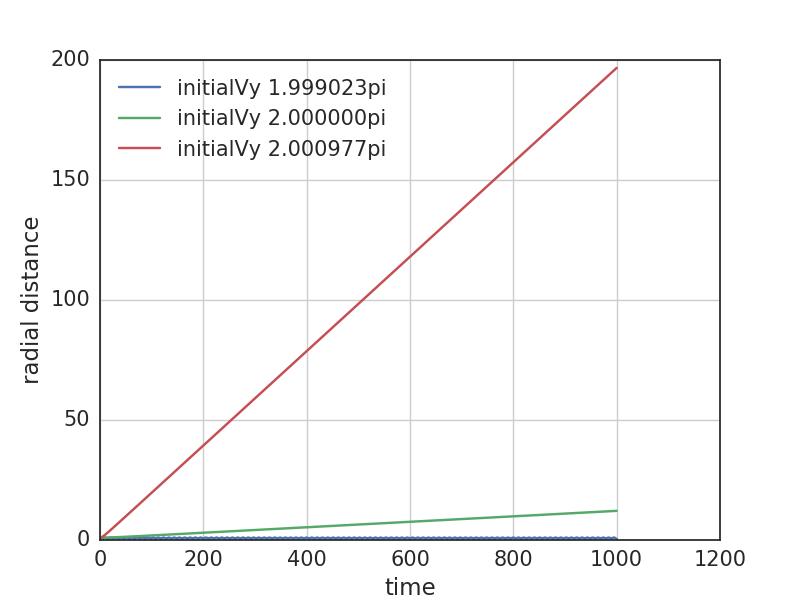
\includegraphics[width=0.99\textwidth]{/home/karl/doc/subj/att/fys4150/project3/resultsKeep/plots/sunEarthradialDistanceVelocityVerletbeta40.png}
		\caption{Sun-Earth system. Alternative force. Escape valocity. $\beta = 3.0$ \\ \textit{We get escape at $v = 2\pi$.}}
		\label{1}
	\end{figure}
\end{minipage}\hfill
\vspace{2ex}

The figures above show that the escape velocities are lowered when the gravitational forces are lowered, as expected.  

\subsection{Center of mass system}
Above we have seen that the solvers reproduce expected behavoiur: Forward Euler does not preserve energy, while Velocity Verlet does, and basic exact results for escapce velocities, energy and angular momentum is well approximated. However, the above was only tested on a two-object system. To check whether the solver works for multibody systems, with more than two objects, a third planet, Jupiter, is added.\\

All the above simulations were based on the assumption that the sun was stationary. This is not the case in reality. To make the solver more realistic, we also introduce movement in the sun by letting the sun be modelled just as the other planets, gravity affecting also the sun's movement. \\

To make the plots easy to interpret, we make sure that the center of mass of the system is stationary. This we do by adjusting the initial velocity of the sun, utilizing the fact that the angular momentum of the system is preserved

\begin{subequations}
	\begin{align}
	0 &= \frac{d \vec R}{dt}	\\
	&= \frac{d}{dt} (\frac{1}{M} \sum_i^{Planets+Sun} m_i \vec{v}_i)\\
	&= \frac{1}{M} \sum_i^{Planets+Sun} m_i v_i \\
	\rightarrow 0 &=m_{sun} \vec{v}_{sun} + \sum_i^{Planets} m_i \vec{v}_i \\
	\vec{v}_{Sun} &= - \frac{\sum_i^{Planets} m_i \vec{v}_i}{m_{Sun}}
	\end{align}
\end{subequations}

The below figures show the results for the three-body systems mentioned above, with fixed and with moving sun, for three different masses of Jupiter.

\begin{minipage}{.3\textwidth} 
	\begin{figure}[H]
		\centering
		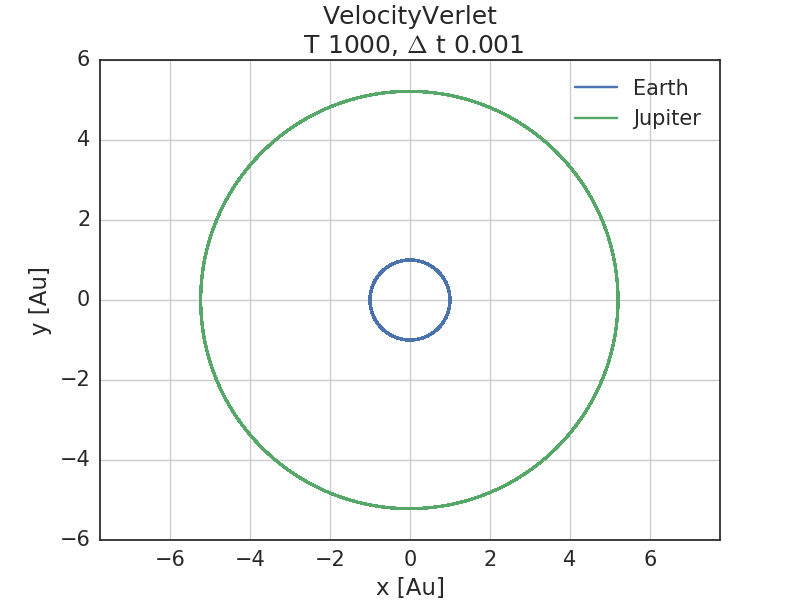
\includegraphics[width=0.99\textwidth]{/home/karl/doc/subj/att/fys4150/project3/resultsKeep/plots/threeBodiesVelocityVerletT1000dt0001.png}
		\caption{3 bodies. Fixed sun. Normal Jupiter mass. \\ \textit{Stable orbits.}}
		\label{1}
	\end{figure}
\end{minipage}\hfill
\begin{minipage}{.3\textwidth} 
	\begin{figure}[H]
		\centering
		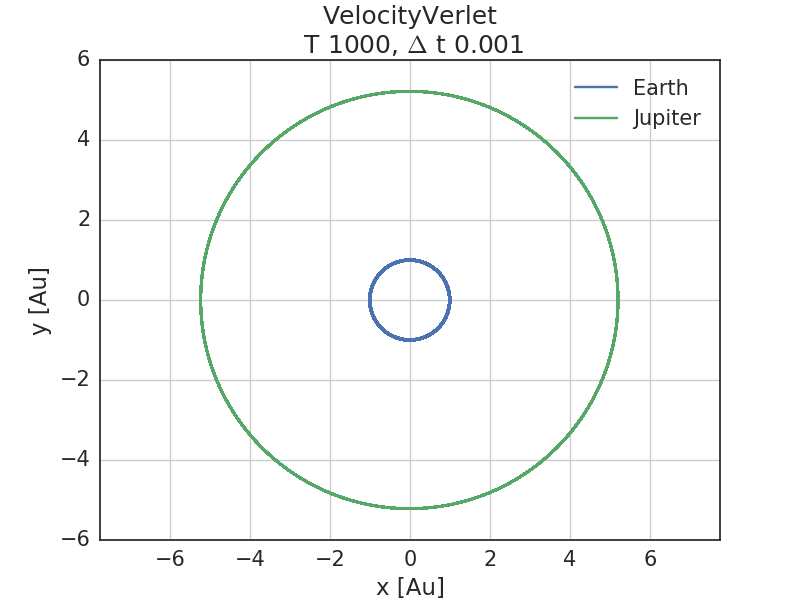
\includegraphics[width=0.99\textwidth]{/home/karl/doc/subj/att/fys4150/project3/resultsKeep/plots/threeBodiesJupiterTimes10VelocityVerletT1000dt0001.png}
		\caption{3 bodies. Fixed sun. Jupiter mass times 10. \\ \textit{Little effect on orbits.}}
		\label{1}
	\end{figure}
\end{minipage}\hfill
\begin{minipage}{.3\textwidth} 
	\begin{figure}[H]
		\centering
		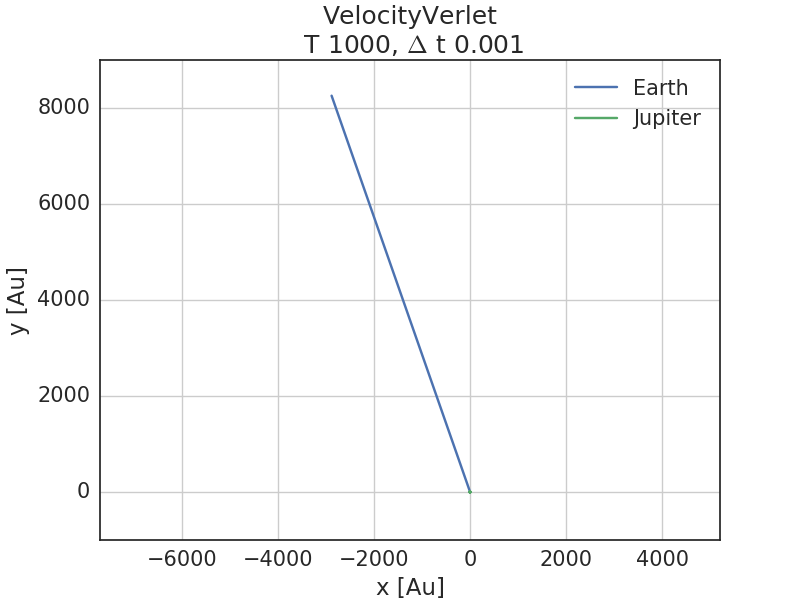
\includegraphics[width=0.99\textwidth]{/home/karl/doc/subj/att/fys4150/project3/resultsKeep/plots/threeBodiesJupiterTimes1000VelocityVerletT1000dt0001.png}
		\caption{3 bodies. Fixed sun.  Jupiter mass times 1000. \\ \textit{Earth escapes.}}
		\label{1}
	\end{figure}
\end{minipage}\hfill
\vspace{2ex}

\begin{minipage}{.3\textwidth} 
	\begin{figure}[H]
		\centering
		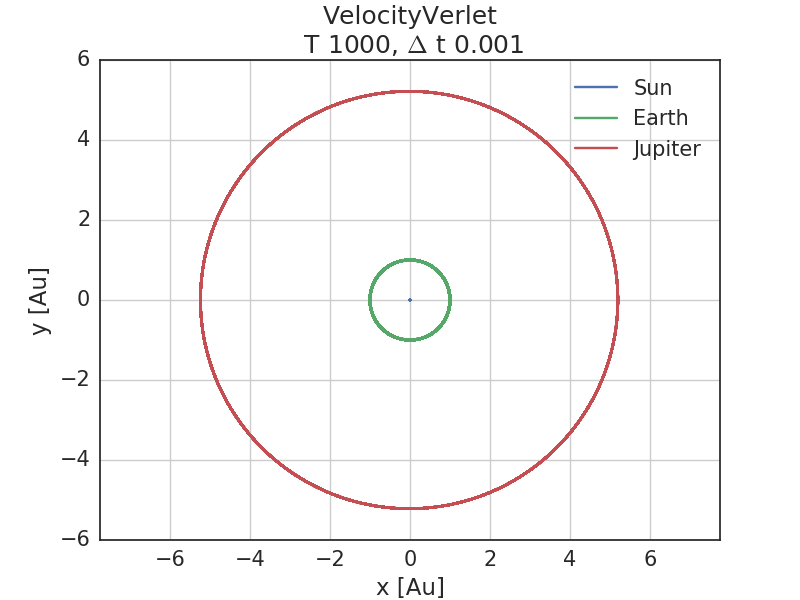
\includegraphics[width=0.99\textwidth]{/home/karl/doc/subj/att/fys4150/project3/resultsKeep/plots/threeBodiesMovingSunVelocityVerletT1000dt0001.png}
		\caption{3 bodies. Moving sun. Normal Jupiter mass. \\ \textit{Stable orbits, as for fixed sun scenario.}}
		\label{1}
	\end{figure}
\end{minipage}\hfill
\begin{minipage}{.3\textwidth} 
	\begin{figure}[H]
		\centering
		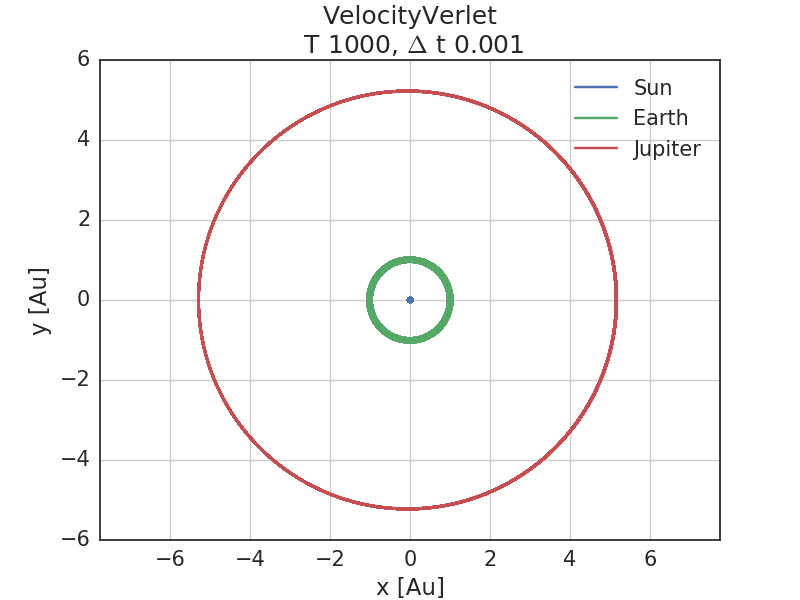
\includegraphics[width=0.99\textwidth]{/home/karl/doc/subj/att/fys4150/project3/resultsKeep/plots/threeBodiesJupiterMassTimes10MovingSunVelocityVerletT1000dt0001.png}
		\caption{3 bodies. Moving sun. Jupiter mass times 10. \\ \textit{Some movement in Sun, but still very similar too fixed Sun scenario.}}
		\label{1}
	\end{figure}
\end{minipage}\hfill
\begin{minipage}{.3\textwidth} 
	\begin{figure}[H]
		\centering
		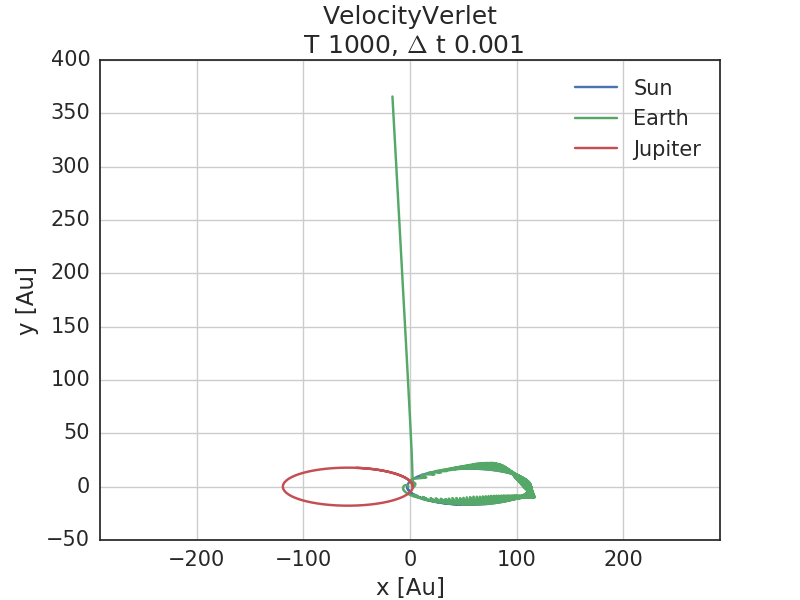
\includegraphics[width=0.99\textwidth]{/home/karl/doc/subj/att/fys4150/project3/resultsKeep/plots/threeBodiesJupiterMassTimes1000MovingSunVelocityVerletT1000dt0001.png}
		\caption{3 bodies. Moving sun.  Jupiter mass times 1000. \\ \textit{Large movement in the Sun. Earth escapes.}}
		\label{1}
	\end{figure}
\end{minipage}\hfill
\vspace{2ex}

The first row in the figures above shows that the solver works for 3 body systems, but also that the Earth escapes in the case where Jupiter's mass equals the Sun' mass.\\

The 2nd row in the figures above shows the solutions for different masses of Jupiter in the case where the Sun is moving. We see that the solution for the two lowest masses of Jupiter resembles the fixed sun scenarios in the 1st row of the above figures. For the case where the mass of Jupiter equals the mass of Sun, however, the solution is quite different in the case with moving sun compared to a fixed Sun. The earth still escapes, but now the Sun moves a lot, which is natural given Jupiter's mass equals the Sun's mass. \\

We have made movies where one can see that the center of mass seems fixed in the moving sun system. To run the movies, simply write "animate threeBodiesMovingSunJupiter1000.mp4" for the moving Sun case, and "animate threeBodiesFixedSunJupiter1000.mp4" for the fixed Sun case. \textbf{Note to instructors:} Somehow we do not succeed in uploading the mp4-files to Github. They are not listed in gitignore, so we do not know why this is. The files are less than 150 kb, so space should not be an issue. Send us an e-mail if you want to check the movies.


\subsection{Solar system}
Since the solver is producing reasonable results for the three-body system, we are now ready to simulate the full solar system. Since we are using classes, going from three objects to ten objects constitutes nearly no work at all! We read in all planets from file in a loop, and use the same method as earlier for adding planets. That is all. The below figures displays the results for the full solar system, with a moving sun. \\


\begin{minipage}{.45\textwidth} 
	\begin{figure}[H]
		\centering
		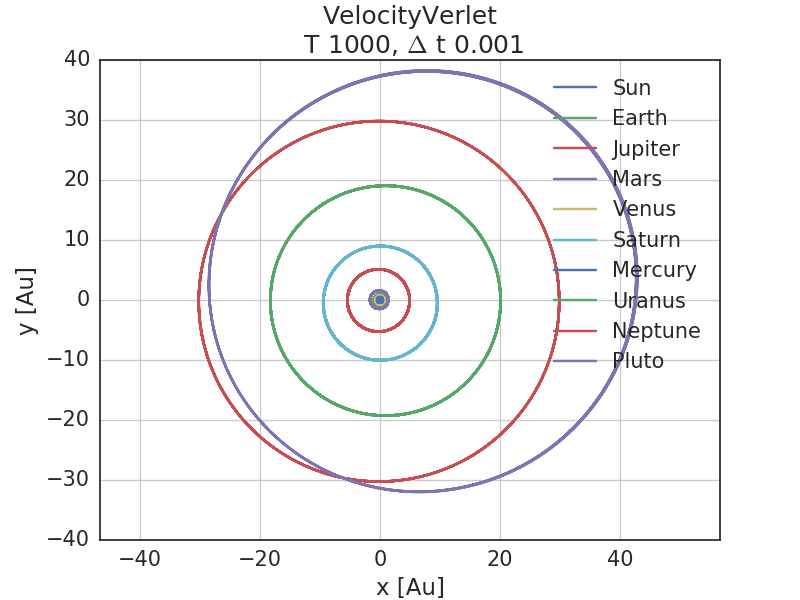
\includegraphics[width=0.99\textwidth]{/home/karl/doc/subj/att/fys4150/project3/resultsKeep/plots/solarSystemMovingSunVelocityVerletT1000dt0001.png}
		\caption{Solar System. Moving sun. All planets 1000 years  \\ \textit{Orbits looks reasonable.}}
		\label{1}
	\end{figure}
\end{minipage}\hfill
\begin{minipage}{.45\textwidth} 
	\begin{figure}[H]
		\centering
		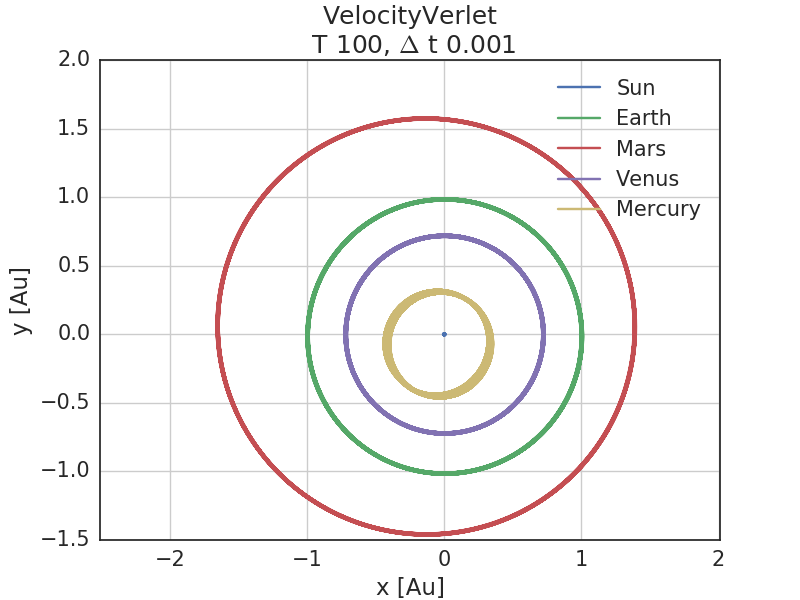
\includegraphics[width=0.99\textwidth]{/home/karl/doc/subj/att/fys4150/project3/resultsKeep/plots/solarSystemMovingSunVelocityVerletT100dt0001.png}
		\caption{Solar System. Moving sun. Inner most planets. 100 years  \\ \textit{Large perihelion precession of Mercury.}}
		\label{1}
	\end{figure}
\end{minipage}\hfill
\vspace{2ex}

The above figure shows that the program nicely simulates the basic dynamics of the solar system. This is as expected, since the most significant forces are included in the program. However, the right figure shows an unnatural movement for Mercury, displaying an unaturally large perihelion precession. This has to do with the ommission of the relativistc correction term in the graviational force. See next section for more on this.

\subsection{Perihelion precession}
Perihelion is the closest point between a planet and sun during one rotation. This precession is supposed to be very small, 43 arcseconds over a century. Since the solver is working so well, we now want to try to reproduce the observed perihelion precession of Mercury by adding a relativistic gravitational term,$\frac{GM_{Sun} M_{Mercury}}{r^2} \frac{3l^2}{r^2c^2}$, where $l = |\vec{r} \times \vec{v}|$, in Mercury's acceleration term.  \\

We implement the relativistic term by creating a new class, "PlanetGeneralRelativityForce", which inherits everything from the Planet class. The acceleration function is corrected by overrideing it in the new class. The new correction term is scaled in the same way as the other terms, and we  end with an acceration equation of type $a = Uncanged(1 + ScaledCorrection)$. \\

We use only two objects for this simulation ,the sun and Mercury. We solve this problem with a stationary sun, and with a moving Sun. We saw that in the three body system, with larger planets than Mercury, the effect of introducing a moving sun was neglieble. However, now we are trying to identify small effects, so the effect of a moving Sun might not be unimportant anymore. \\

We assume initial position of Mercury at perihelion, and localize perihelion at $(x,y) = (0.3075 Au, 0)$. Initial velocity is set to 12.44 $Au/Yr$. When doing this, we get the following results for the perihelion precession for different $\Delta t$.\\

\begin{figure}[H]
	\centering
	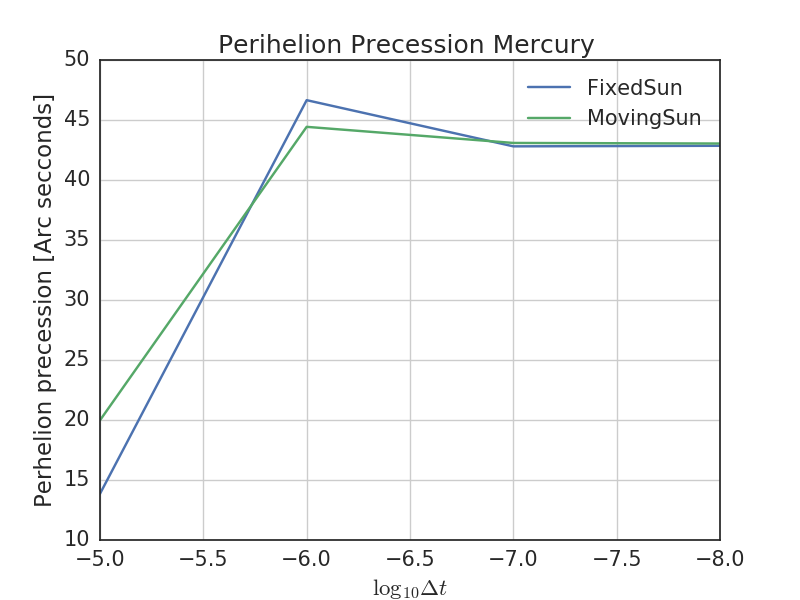
\includegraphics[width=0.6\textwidth]{/home/karl/doc/subj/att/fys4150/project3/resultsKeep/plots/Perihelion.png}
	\caption{Perihelion precession Mercury . \\ \textit{The fixed sun and moving Sun approximatins both converges, the moving sun approximation closest to the observed value}}
	\label{1}
\end{figure}

The above suggests that the solver is able to predict the perihelion precession of Mercury well. The reuslts for the precesions for $\Delta t = 10^{-8}$ is $42.85$ and $43.04$ for fixed and moving sun respectively, suggesting that applying a real center of mass system, as the moving sun system, gives better approximations for fine effects like Mercury's perihelion precession.

\section{Conclusions}
In this project we solve problems for planetary motion, which mathematically are systems of 2nd order differential equations. To make the equations easier to work with, we scale the equations to astronomical units.\\

The systems of 2nd order equations are reformulated to systems of 1st order equations by use of variable substitution. \\

Solving the large system of equations in C++, we take apply classes and class inheritance.\\

Two numerical methods are used: the forward Euler method and the Velocity Verlet method. We show that the velocity Verlet method reproduces physical results like conservation of energy and angular momentum well, while the Forward Euler method does not reproduce these results as well. The Velocity Verlet method converges twice as fast to correct solutions, for preservation of energy and angular momentim, compared to the Forward Euler method. Both methods gives bad results for the largest time steps. The methods are shown to involve approximatly the same amount of FLOPS.\\

The Velocity Verlet method reproduces the exact terminal velocity of a two object sun-earth system. Velocity Verlet also gives reasonalbe physical results in scenarios where the gravitational force is changed. \\

Adding a third planet, Jupiter, to the stationary Sun earth system, gives reasonable results using Velocity Verlet: the orbits stay circular and stable. Also here the largest time steps give strange results, while the finer time steps gives convergent solutions. Making Jupiter's mass equal to the Sun's mass makes the earth escape. More realistic scenarios, that includes movement in the sun, keeping the center of mass of the system constant, produces reasonable results: When Jupiter's mass is enlarged, the sun starts to move. The center of mass seems to be fixed.\\

The full solar system is simulated with the Velocity Verlet solver and with movement in the sun. Except for Mercury's behaviuour, the results seems reasonable, all other orbits being stable.\\

By adding a relativistic correction to the gravitational force from sun on Mercury, the perihelion precession of Mercury around the sun is not fully reproduced. Both in the cases with a fixed Sun and with a moving Sun we get a Perihelion precesion of 43 arc secconds. The results converge, meaning that the perihelion procession result stabilizes for the finest time steps. \\

For future reference, we add the we could have improved the speed of the solvers by taking into account that the gravitational force between two planets are equal in magnitude. Taking this into account in the force calculations, we could have halved the number of FLOPS!


\section{Feedback}
\subsection{Project 1}
This project has been extremely educational. We learned about about c++, especially pointers and dynamic memory allocoation. Also which for us was a well forgotten subject, we learned about dangerous of numerical round-off errors. \\

We feel the size of the project is large, much larger than typical assignments in other courses. However, the quality and quantity of the teaching without a doubt made the workload managable. The detailed lectures, combined with the fast and good respones on Piazza helped a lot!\\

We think the project could have gone even smoother, if we on the 2nd lab-session had learned basic branching in Github. We used a considerable amount of time finding out of this.\\

All in all, two thumbs up!

\subsection{Project 2}
\begin{itemize}
	\item  catch: We ended up using a lot of time making this work properly. Still we have some problems with catch and Qt. We think we might had benefited from a demonstration at the lab.
	
	\item We were not able to understand the revised Sturm-Bisection algorithm from Barth et al.'s \cite{barth} paper on the revised Sturm-Bisection. 
	
	\item Apart from the small details above, we are very happy about this project. How would have thought linear algebra could be fun?!
\end{itemize}

\subsection{Project 3}
\begin{itemize}
	\item  Classes: Very useful!
	
	\item Extra fun working with a system that one "knows" a little bit about. Also easier to judge the quality of the results, and find potential errors.
\end{itemize}













\pagebreak
\begin{thebibliography}{9}
	\bibitem{MHJ} 
	Hjorth-Jensen, M.(2015)
	Computational physics. Lectures fall 2015. 
	\url{https://github.com/CompPhysics/ComputationalPhysics/tree/master/doc/Lectures}
	

	


\end{thebibliography}


\end{document}
